%
% DS 5110 (Blue Team) Project Proposal
%
\documentclass[12pt]{article}

%
% Packages
%
\usepackage{amsmath}
\usepackage{enumerate}
\usepackage[utf8]{inputenc}

\RequirePackage{graphics}

\usepackage{graphicx}
\graphicspath{ {imgs/} }

%
% Document Settings
%
\setlength{\parskip}{1pc}
\setlength{\parindent}{0pt}
\setlength{\topmargin}{-3pc}
\setlength{\textheight}{9.5in}
\setlength{\oddsidemargin}{0pc}
\setlength{\evensidemargin}{0pc}
\setlength{\textwidth}{6.5in}

\title{DS 5110: Project - Fall 2017}
\author{Tyler Brown, Sicheng Hao, Nischal Mahaveer Chand, Sumedh Sankhe}
\date{ }


% START DOCUMENT
\begin{document}

\maketitle

\section{Summary}

The City of Boston provides an open data platform, Analyze Boston, 
containing information related to our lives in the city. Property 
assessment data from 2014-2017 is one of the resources available on their
 open data platform. Included in the property assessment data is 
"property, or parcel, ownership together with information about value, 
which ensures fair assessment of Boston taxable and non-taxable property 
of all types and classifications" (Citation of dataset here). Our team 
has aggregated each available year to create a time series dataset of 
Property Assessments in Boston. This aggregated dataset allows us to 
provide unique insights into property valuations and ownership strategies.

The problem our group focusing is how can we identify top performing 
property owners to demonstrate the dominant strategy to new buyers? Build
 a Shiny App to help people visualize our findings of house price in each
 neighborhood as well as where is housing value increase the most. 

\section{Proposed Plan of Research}

 The datasets we are having right now are separate yearly. The first step 
we are going to do is merge them into one single file. Then we are going 
to do some necessary cleaning for the data set. 

In the second step, we are going to filter out the data that could 
represent the problem we are trying to solve. Maybe add some data from 
other sources( like Google Maps or Zillow)

To help people understand the data better. In the last step we will make 
an interactive Shiny application to visualize our finding. 


\section{Preliminary Results}

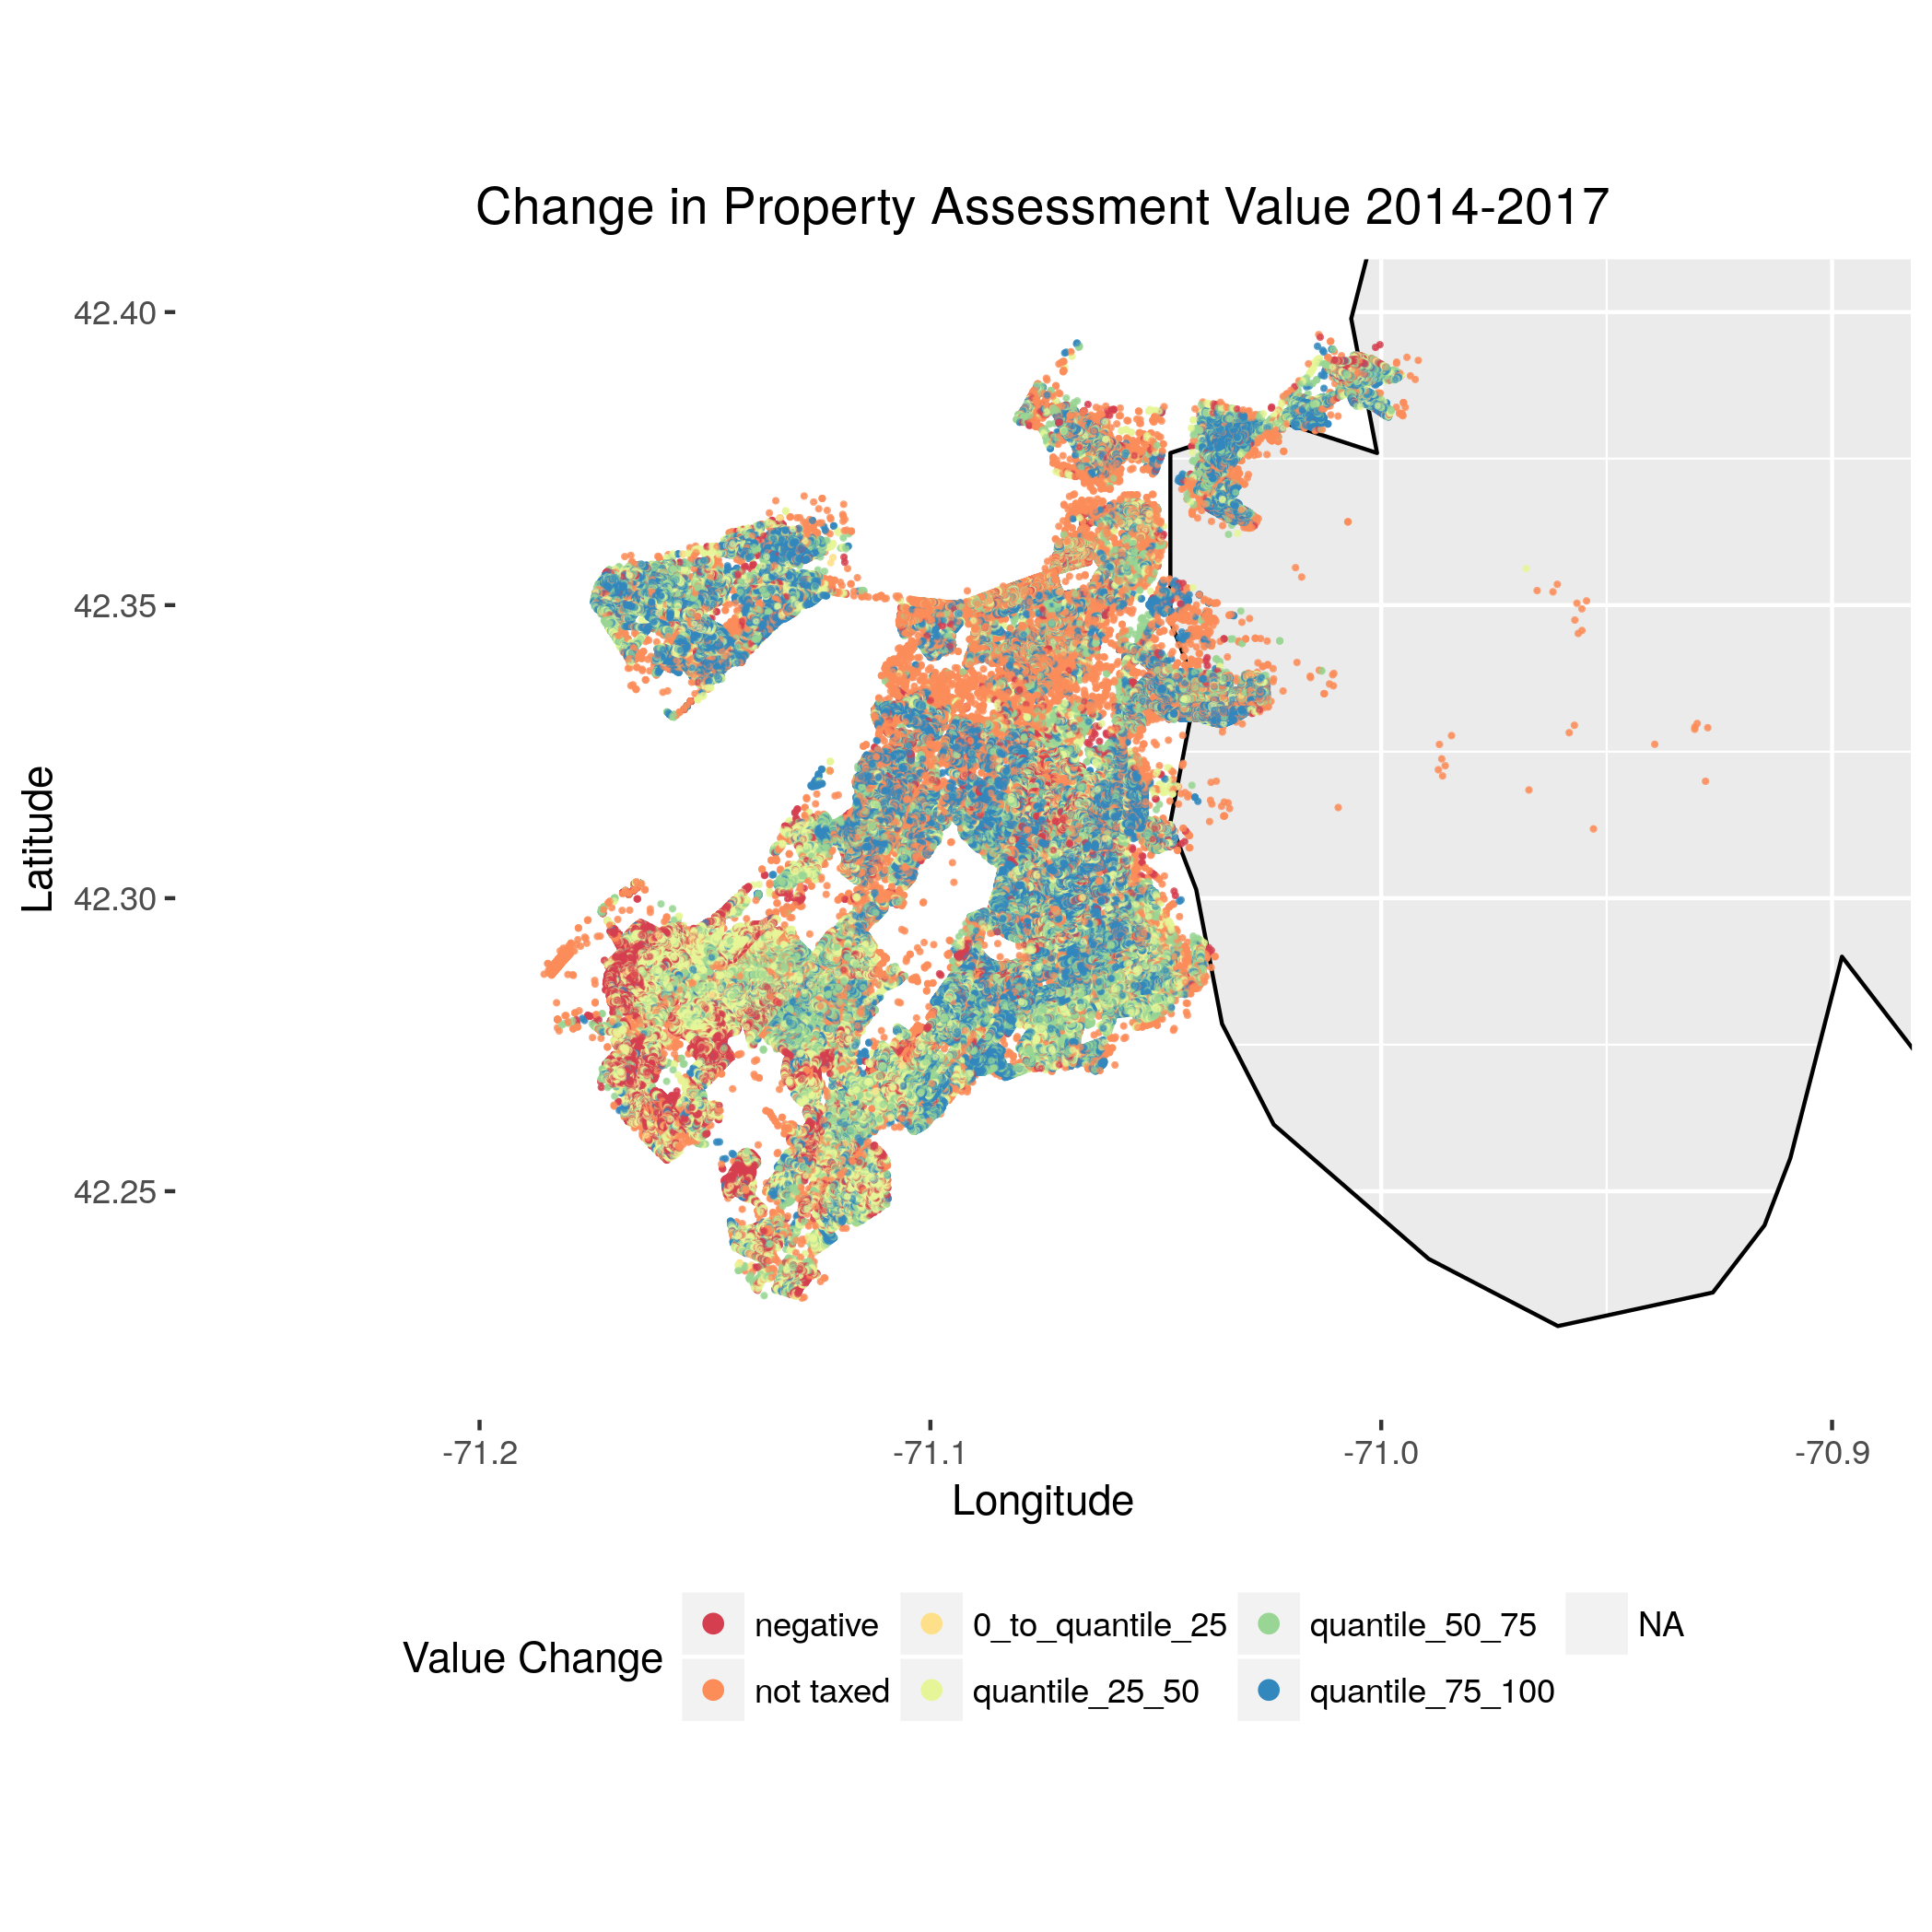
\includegraphics[scale=0.85]{property_delta2014-2017}


\bibliography{references} 
\bibliographystyle{apalike}

\end{document}
